\documentclass[oneside,a4paper,14pt]{extarticle}

\usepackage[T2A]{fontenc}
\usepackage[top=20mm,bottom=20mm,left=30mm,right=10mm]{geometry}
\usepackage[utf8]{inputenc}
\usepackage[russian]{babel}
\usepackage{textcomp}
\usepackage{indentfirst}
\usepackage{graphicx}
\usepackage{mwe}
\usepackage{wrapfig}
\usepackage{caption}
\usepackage{amsmath}
\usepackage{amsfonts}
\usepackage{amsthm}
\usepackage[all]{xy}
\usepackage[breaklinks]{hyperref}
\usepackage{titlesec}
\usepackage{listings}
\usepackage{minted,fancyvrb}

\setminted{style=rainbow_dash,fontsize=\small}

\titleformat{\section}
{\normalsize\bfseries}
{\thesection}{1em}{}
\titleformat{\subsection}
{\normalsize\bfseries}
{\thesubsection}{1em}{}
\titleformat{\subsubsection}
{\normalsize\bfseries}
{\thesubsubsection}{1em}{}

\renewcommand\baselinestretch{1.33}\normalsize
\setlength{\parindent}{1.25cm}

\begin{document}
\newpage\thispagestyle{empty}

\begin{center}
МИНИСТЕРСТВО НАУКИ И ВЫСШЕГО ОБРАЗОВАНИЯ\\
РОССИЙСКОЙ ФЕДЕРАЦИИ\\
ФЕДЕРАЛЬНОЕ ГОСУДАРСТВЕННОЕ БЮДЖЕТНОЕ\\
ОБРАЗОВАТЕЛЬНОЕ УЧРЕЖДЕНИЕ ВЫСШЕГО ОБРАЗОВАНИЯ\\
«ВЯТСКИЙ ГОСУДАРСТВЕННЫЙ УНИВЕРСИТЕТ»\\
Институт математики и информационных систем\\
Факультет автоматики и вычислительной техники\\
Кафедра электронных вычислительных машин
\end{center}

\vspace{30mm}

\begin{center}
Отчёт по лабораторной работе № 2.1\\
по дисциплине\\
«Управление данными»\\
«Основы DML-запросов в PostgreSQL»
\end{center}

\vspace{40mm}

\noindent
\begin{tabular}{l r}
Выполнил студент гр. ИВТб-2303-06-00 \hspace{3mm}\rule[-1mm]{20mm}{0.15mm} /Перевозчиков Д.А./ \\

Проверил \hspace{57mm}\rule[-1mm]{20mm}{0.15mm} /Клюкин В. Л./
\end{tabular}

\vfill
\begin{center}
Киров\\
2026
\end{center}

\newpage\thispagestyle{empty}

\section{Цели лабораторной работы}

\begin{itemize}
    \item освоить основные варианты DML-запросов в PostgreSQL;
    \item научиться создавать SQL-скрипты для заполнения таблиц данными;
    \item научиться использовать команды \texttt{UPDATE} и \texttt{DELETE};
    \item научиться работать с представлениями.
\end{itemize}

\section{Задание}

Для выполнения лабораторной работы используется база данных, созданная в лабораторной работе № 1. Необходимо выполнить следующие задания:

\begin{enumerate}
    \item Создать и выполнить SQL-скрипт заполнения таблиц данными с помощью команды \texttt{INSERT}.
    \item Создать и выполнить SQL-скрипт изменения существующих записей с помощью команды \texttt{UPDATE}.
    \item Создать и выполнить SQL-скрипт удаления записей с помощью команды \texttt{DELETE}.
    \item Создать и выполнить SQL-запросы для получения данных с помощью команды \texttt{SELECT}, используя различные условия, сортировку, ограничения количества строк, подзапросы и соединения таблиц.
    \item Создать представления, объединяющие информацию из нескольких таблиц, и выполнить выборки из созданных представлений.
\end{enumerate}

\newpage
\section{Решение}

\subsection{Задание 1. Заполнение таблиц данными}

В лабораторной работе № 1 была разработана структура базы данных для хранения информации о ресурсах гоночного клуба. База данных содержит таблицы \texttt{car}, \texttt{trainer}, \texttt{trainer\_car}, \texttt{competition} и \texttt{achievement}.

Для проверки разработанной структуры и последующего выполнения запросов необходимо заполнить таблицы тестовыми данными.

Для заполнения таблиц был разработан SQL-скрипт. Данные добавляются в таблицы автомобилей, тренеров, специализаций тренеров, соревнований и достижений тренеров.

Полный текст SQL-скрипта заполнения таблиц представлен в Приложении А1.

\subsection{Задание 2. Изменение существующих записей}

Для изменения данных в существующих записях использована команда \texttt{UPDATE}. Она позволяет изменить значения одного или нескольких столбцов у строк, удовлетворяющих условию, заданному в предложении \texttt{WHERE}.

В разработанном скрипте реализованы следующие операции:

\begin{itemize}
    \item изменение названия соревнования «Ралли Монте-Карло»;
    \item изменение даты проведения соревнования «Ралли Уэльс»;
    \item изменение занятого места в таблице достижений тренера;
    \item изменение банковского счёта тренера;
    \item изменение URL фотографии автомобиля;
    \item изменение цвета автомобиля Audi Quattro;
    \item перевод автомобиля ОКА в состояние утилизации;
    \item изменение специализации тренера путём замены автомобиля ОКА на Porsche 911.
\end{itemize}

Полный текст SQL-скрипта изменения данных представлен в Приложении А2.

\subsection{Задание 3. Удаление существующих записей}

Для удаления записей из базы данных использована команда \texttt{DELETE}. Условия удаления задаются с помощью предложения \texttt{WHERE}.

В разработанном скрипте предусмотрены следующие операции:

\begin{itemize}
    \item удаление специализации тренера Сергея Кузнецова на автомобиле Audi RS2;
    \item удаление автомобиля Tesla Model S;
    \item удаление тренера Сергея Кузнецова;
    \item удаление соревнования «Ралли Австралия».
\end{itemize}

В запросах используются условия, позволяющие определить удаляемые записи по характеристикам сущностей. Для удаления специализации применяются подзапросы, позволяющие получить идентификаторы тренера и автомобиля.

Полный текст SQL-скрипта удаления данных представлен в Приложении А3.

\subsection{Задание 4. Получение данных с помощью команды SELECT}

\textbf{1. Сортировка и ограничение количества строк.}

Для получения первых десяти автомобилей в алфавитном порядке используется сортировка по столбцу \texttt{title} и ограничение результата с помощью \texttt{LIMIT}.

\textbf{2. Соединение таблиц.}

Для поиска трёх тренеров, специализирующихся на автомобиле Mazda MX-5 Miata, используются таблицы \texttt{trainer}, \texttt{trainer\_car} и \texttt{car}. Соединение выполняется по идентификаторам связанных записей. Результат сортируется по фамилии тренера.

\textbf{3. Использование OFFSET.}

Для поиска второго по возрасту тренера записи сортируются по году рождения по возрастанию. С помощью \texttt{OFFSET 1} пропускается первая запись, а \texttt{LIMIT 1} ограничивает результат одной строкой.

\textbf{4. Фильтрация по условию.}

Для получения автомобилей мощностью более 100 лошадиных сил, которые не находятся в утилизации, используется условие \texttt{WHERE} с двумя логическими выражениями, объединёнными оператором \texttt{AND}.

\textbf{5. Объединение результатов запросов.}

Для получения списка победителей и призёров соревнования «Кубок Поршня» применяется оператор \texttt{UNION}. Первый запрос выбирает участников, занявших первое место, а второй получает остальные призовые места. В результирующей выборке дополнительно выводится статус участника.

\textbf{6. Поиск по шаблону.}

Для поиска тренеров с фамилиями, начинающимися на букву «И», используется оператор \texttt{LIKE} с шаблоном \texttt{'И\%'}. Символ \texttt{\%} обозначает произвольную последовательность символов.

\textbf{7. Группировка и фильтрация групп.}

Для поиска тренеров, специализирующихся ровно на одном автомобиле, используются \texttt{GROUP BY}, агрегатная функция \texttt{COUNT} и условие \texttt{HAVING}. В результате остаются только группы, количество автомобилей в которых равно единице.

\textbf{8. Использование подзапроса.}

Для поиска автомобилей мощностью выше средней по автопарку применяется подзапрос с агрегатной функцией \texttt{AVG}. Сначала вычисляется средняя мощность автомобилей, затем выбираются машины, мощность которых превышает полученное значение.

\textbf{9. Выборка с использованием подзапроса.}

Для поиска тренеров, любимые автомобили которых имеют мощность более 300 лошадиных сил, используется подзапрос к таблице \texttt{car}. Идентификаторы подходящих автомобилей сравниваются со значениями столбца \texttt{favorite\_car\_id} таблицы \texttt{trainer}.

Полный текст SQL-скрипта выборок представлен в Приложении А4.

\subsection{Задание 5. Создание представлений}

Представление (\texttt{VIEW}) представляет собой виртуальную таблицу, позволяющую сохранять сложные запросы и повторно использовать их для получения информации без необходимости каждый раз записывать соединения и вычисления заново.

Для базы данных гоночного клуба созданы пять представлений.

\textbf{1. Представление \texttt{v\_trainer\_info}.}

Представление содержит основную информацию о тренерах и их любимых автомобилях. С помощью \texttt{LEFT JOIN} объединяются таблицы \texttt{trainer} и \texttt{car}.

\textbf{2. Представление \texttt{v\_competition\_results}.}

Представление предназначено для получения информации о результатах участия тренеров в соревнованиях. С помощью \texttt{INNER JOIN} объединяются таблицы \texttt{competition}, \texttt{achievement} и \texttt{trainer}.

\textbf{3. Представление \texttt{v\_car\_full}.}

Представление содержит сведения об автомобилях и агрегированную информацию об их использовании.

Для подсчёта количества тренеров используется \texttt{COUNT(DISTINCT ...)}, позволяющая исключить повторный подсчёт одного тренера. Для объединения фамилий применяется агрегатная функция \texttt{STRING\_AGG}.

\textbf{4. Представление \texttt{v\_trainer\_rating}.}

Представление предназначено для получения статистики достижений тренеров. Для каждого тренера определяется общее количество достижений и количество первых мест.

Для вычисления показателей используются \texttt{COUNT} и агрегатная функция с фильтром \texttt{FILTER (WHERE ...)}. Применение \texttt{LEFT JOIN} позволяет включать в результат тренеров, у которых отсутствуют достижения.

\textbf{5. Представление \texttt{v\_competition\_full}.}

Представление предназначено для получения сводной информации о соревнованиях. Для каждого соревнования определяется количество участников из автоклуба и формируется список фамилий тренеров, участвовавших в соревновании.

Полный текст SQL-скрипта создания представлений представлен в Приложении А5.

\subsection{Проверка работы представлений}

После создания представлений выполнены запросы для получения данных из них.

Из представления \texttt{v\_car\_full} получен список автомобилей, их состояние утилизации, количество тренеров, использующих автомобиль, и фамилии тренеров, для которых автомобиль является любимым.

Из представления \texttt{v\_trainer\_info} получена информация о тренерах и характеристиках их любимых автомобилей.

Из представления \texttt{v\_competition\_full} получена сводка по соревнованиям, включающая даты проведения, количество участников и список фамилий.

Из представления \texttt{v\_competition\_results} получены результаты соревнований с указанием тренеров и занятых мест.

Из представления \texttt{v\_trainer\_rating} получена статистика достижений тренеров, включающая общее количество достижений и количество побед.

Результаты выполнения запросов к представлениям представлены на рисунках 1--5.

\begin{figure}[h!]
    \centering
    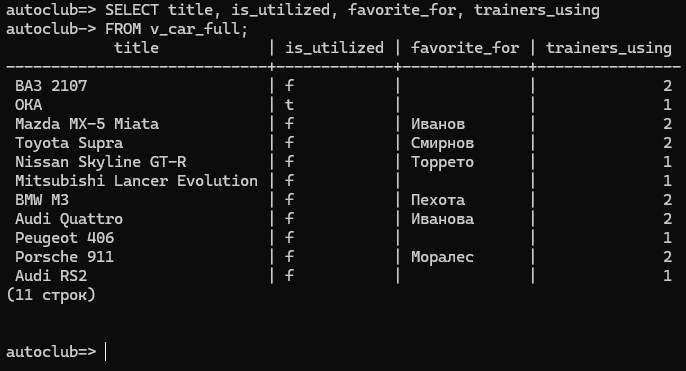
\includegraphics[width=0.85\textwidth]{images/v_car_full}
    \caption*{Рисунок 1 -- Результат выборки из представления \texttt{v\_car\_full}.}
\end{figure}

\begin{figure}[h!]
    \centering
    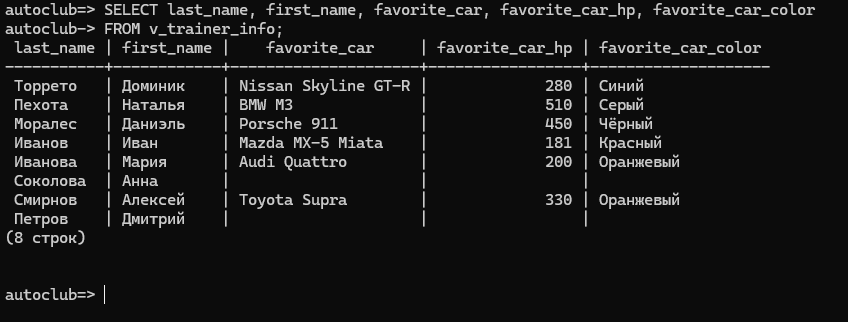
\includegraphics[width=0.85\textwidth]{images/v_trainer_info}
    \caption*{Рисунок 2 -- Результат выборки из представления \texttt{v\_trainer\_info}.}
\end{figure}

\begin{figure}[h!]
    \centering
    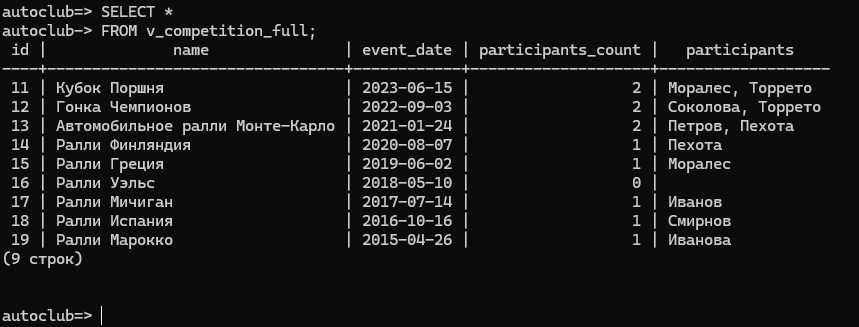
\includegraphics[width=0.85\textwidth]{images/v_competition_full}
    \caption*{Рисунок 3 -- Результат выборки из представления \texttt{v\_competition\_full}.}
\end{figure}

\begin{figure}[h!]
    \centering
    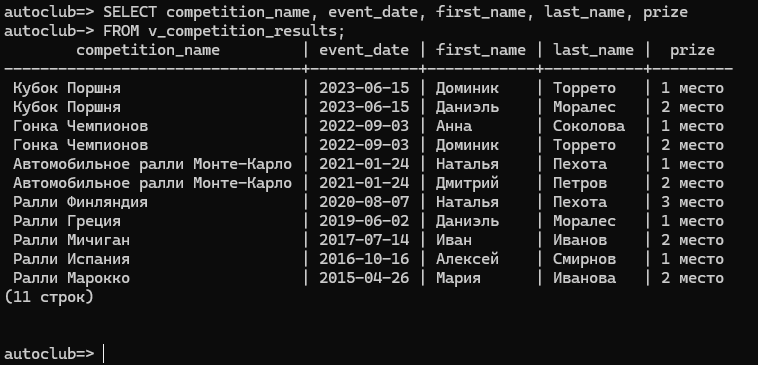
\includegraphics[width=0.85\textwidth]{images/v_competition_results}
    \caption*{Рисунок 4 -- Результат выборки из представления \texttt{v\_competition\_results}.}
\end{figure}

\begin{figure}[h!]
    \centering
    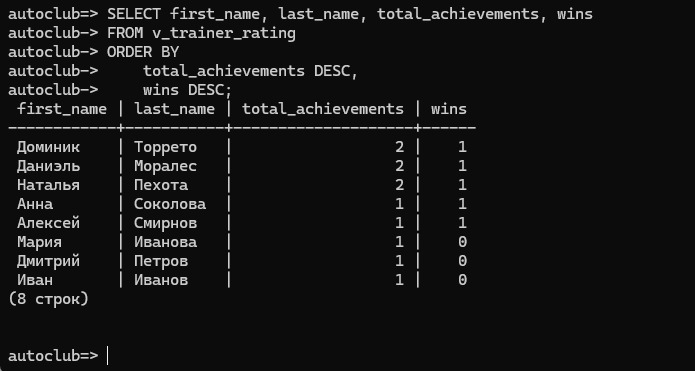
\includegraphics[width=0.85\textwidth]{images/v_trainer_rating}
    \caption*{Рисунок 5 -- Результат выборки из представления \texttt{v\_trainer\_rating}.}
\end{figure}

\section*{Вывод}

В ходе выполнения лабораторной работы были освоены основные способы манипулирования данными в PostgreSQL. Разработаны SQL-запросы для добавления, изменения, удаления и получения записей из таблиц базы данных гоночного клуба.

В процессе выполнения работы использованы фильтрация, сортировка, ограничение количества строк, соединения таблиц, объединение результатов запросов, подзапросы и агрегатные функции. Созданы представления для получения сводной информации об автомобилях, тренерах, соревнованиях и достижениях.

В результате работы закреплены навыки написания DML-запросов и создания представлений, позволяющих получать осмысленную информацию из нескольких связанных таблиц.

\newpage
\begin{flushright}
\bf Приложения
\end{flushright}

\section*{Приложение А1}
Исходный код запросов для заполнения таблиц данными:
\inputminted{sql}{../insert.sql}

\newpage
\section*{Приложение А2}
Исходный код запросов для изменения данных:
\inputminted{sql}{../update.sql}

\newpage
\section*{Приложение А3}
Исходный код запросов для удаления данных:
\inputminted{sql}{../delete.sql}

\newpage
\section*{Приложение А4}
Исходный код запросов для выборки данных:
\inputminted{sql}{../select.sql}

\newpage
\section*{Приложение А5}
Исходный код запросов для создания представлений:
\inputminted{sql}{../view.sql}

\end{document}
